\chapter{\uppercase{Preliminaries}
\footnote{Portions of this chapter are based on an earlier work:
A geographic study of tie strength in social media, in
Proceedings of the 20th ACM international conference on Information and
knowledge management, \copyright ACM, 2011.
http://dx.doi.org/10.1145/2063576.2063959}
}

\flsec{Definitions}

Before going into the details of the data collection, we first define a few
terms to simplify the process of explaining how the data was collected.
%
Figure~\ref{fig:Terms} shows a social graph and uses most of the terms
defined in this section.
%
\textbf{Contacts} are defined to be the set of a user's friends, followers, and
people who a user mentioned in her tweets (i.e., people the user speaks to).
%
Since Twitter does not provide a mechanism to determine who mentioned a given
user, only one-directional conversation is considered.
%
In some blogging platforms, such as Tumblr, it is relatively easy to find the
communication edges that point back toward a user.
%
In those platforms, it would be fairly straightforward to use that information
in location prediction.

\begin{figure}[tbh]
\centering
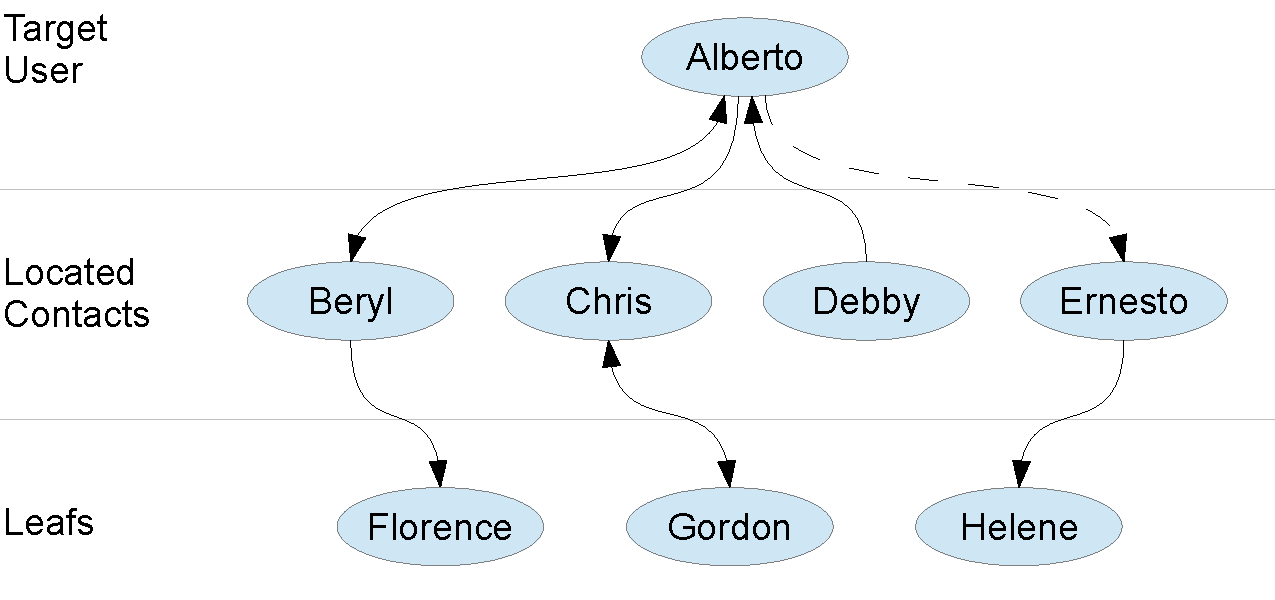
\includegraphics[width=\linewidth]{figures/terms.pdf}
\caption{
A small sample social graph for illustrating definitions used in this paper.
Alberto adds location information to his tweets.
Beryl is a reciprocal friend of Alberto, Chris is just a friend since Alberto
follows Chris, Debby is just a follower, and Ernesto is just mentioned.
The line to Ernesto is dashed to show that there is no friend/follow
relationship between Alberto and Ernesto.
The other arrows show who follows whom.
}
\label{fig:Terms}
\end{figure}

Any given contact can be categorized into precisely one of these four disjoint
sets:
\begin{description}
\item[Reciprocal Friend] The target user follows this user and is followed
    back.
\item[Just Friend] The target user follows this user and is not followed
    back.
\item[Just Follower] The target user is followed by this user, but does
    not follow them.
\item[Just Mentioned] The users do not follow each other, but the target
    user mentioned the name of the other user in a tweet.
\end{description}

%Our crawler starts from a set of seed users and goes two steps out on the
%social graph.
%
%We created labels for the seed users and each of the steps along the way:
%
%\begin{description}
%\item[geo-located users] These users choose to use Twitter's location sharing
%    features, which means that we have precise latitude and longitude
%    coordinates for their location.
%\item[target users] These are a randomly chosen subset of the geo-located users
%    who have at least one contact.
%\item[geocoder calibration users] These are geo-located users who filled out their
%    location field with a location we could decode, but were not selected to be
%    part of the target users. They are used to differentiate between
%    high-quality locations and low-quality locations that are likely to be
%    wrong.
%\item[located contacts] These are the 25 randomly chosen contacts of
%    target users who have locations that we can decode.
%\item[leaves] These are at most 100 of the contacts of the located contacts.
%    When we selected leaves, we excluded the target users from the contacts so
%    that the distances to contacts would be independent from the distances to
%    leaves.
%\end{description}

%\jam{define things in math notation here}


\begin{table*}[tb]
\scriptsize
\centering
\begin{tabular}{l l p{4cm} p{6cm}}
    Label & Size & Description & Data obtained \\
    \hline
    Target Users & 249,584 & Users who posted at least 3 geo-located tweets &
    Location from GPS coordinates, user ids of friends and followers,
    and text of tweets. \\
    Geocoded Users & 894,617 & Users who posted at least 3 geo-located tweets
    and had a location the geocoder could parse, but not selected as target users &
    Location from GPS coordinates and geocoded location from user profile \\
    % 10,081,957 located contacts
    Located Contacts & 10 million & 25 contacts of target users with locations, randomly selected &
    Geocoded location from profile, user ids of friends and followers, and text of tweets \\
    % 71,596,805 leafs minus some of 250k contacts
    Leafs & 71 million & 100 contacts of target users, randomly selected &
    user profile (some of these users have a geocoded profile)\\
\end{tabular}
\caption{Four different sets of users and the data we obtained about them}
\label{tab:datasets}
\end{table*}



\flsec{Data collection}
To investigate how social relation and geographical distance between the
relations correlate, we sample a dataset from Twitter.
%
Our analysis and prediction is based on data collected from Twitter during
May, June, and July of 2012.

We built a crawler to find these contacts for users who used Twitter's Location
Feature to disclose their location.
%
The crawler sampled over one hundred million geo-coded tweets by monitoring
Twitter's public streaming API for all of May 2012.
% 118,464,320 lines including keepalive newlines and non-status messages.
We kept the tweets from the users who posted at least three tweets, which left
us with 1,758,101 Twitter users.
%
For each of these users with geo-coded tweets, we used the median latitude and
median longitude of the locations of the user's tweets as an approximation of
her home location.
%
Some Twitter accounts, such as accounts that posted jobs, would
move around faster than a human could possibly move.
%
To account for this, the crawler calculated the distance between each tweet and
the user's home location.
%
The crawler ignored users if the median distance from their tweets to their
home location was greater than 50 miles.
%
This only removed 3.4\% of the geo-located users.
%
We also removed an additional 2.9\% of the geo-located users who did not have
any contacts with locations we could decode, which left us with 1.6 million
Twitter users with a known location.
%
We randomly selected 249,584 of these users for analysis and experimentation.
\footnote{We originally selected 250,000 users, but had to remove 416 of them.
These users had contacts with locations, but none of their contacts had
meaningful locations.}
%
We refer to these users as the target users.
%
Almost all of the experiments in this paper are based on these target
users.

Users who post geo-located tweets are not entirely representative of the
average Twitter user.
%
In particular, they are less concerned about their privacy and have a precise
location.
%
We only use information obtained from the contacts, and not the geo-located
users themselves in our prediction.
%
There are some Twitter accounts, such as large organizations, who do not have a
single location.
%
In practice, a location prediction system would need to identify users who do
not have a location.



%To enable parallelization, we divided those users into 100 groups based on
%the two least significant digits in their Twitter user id, and randomly selected
%2500 users from each of the groups.

% distribution of the contacts
%     med  avg      std
%rfrd 62.0 132.7148 278.394
%jfol 35.0 143.4844 456.629
%jfrd 78.0 153.5700 241.222
%jats  5.0   7.0764   8.060

For all of the target users, the crawler used Twitter's API to download
the users' 100 most recent tweets, a list of friend ids, and a list of follower ids.
%
Most of the target users had plenty of contacts of each of the four types.
%
The median number of reciprocal friends is 62, and the average is 132.
%
The average numbers are higher because the number of contacts a user has
follows a heavy-tailed distribution.
%
The medians for other types of contacts are 35 just followers, 78 just friends,
and 7 just mentioned.
%
If a user had over 25 contacts in any of the four types of contacts, the
crawler chose a random sample of 25 from each of the types of contacts, and
downloaded the profiles for up to 100 total contacts per target user.
%
From that 100, we randomly picked at most 25 contacts with locations we could
decode to be the located contacts. For those located contacts, we downloaded
their friends, followers, and tweets.
%
We finished this process by downloading up to 100 profiles of the contacts of
the contacts.
%
Since the Twitter social network graph has a large strongly connected
component, there are a significant number of users who are contacts or leafs for
more than one target user.
%
In the end, we collected just over 73 million Twitter user profiles.
%
Table~\ref{tab:datasets} shows a summary of the data obtained from Twitter.

\flsec{Geocoding}
We use Gisgraphy\footnote{\url{http://www.gisgraphy.com/}} to do geocoding.
%
Gisgraphy does full-text search on the
GeoNames\footnote{\url{http://www.geonames.org/}} database using Lucene.
%
Since it runs locally, it is not limited to a certain number of queries per day.
%
Gisgraphy's geocoder returns ranked results based on a full text search
over millions of geographical features such as countries, cities, and schools.

The location field on a user's profile is just a text field that asks the user
to respond to ``Where in the world are you?''.
%
Responses vary from precise latitude and longitude coordinates entered
automatically by smartphone apps to jokes and nonsense.
%
Our system does some preprocessing before sending user-submitted locations to
the geocoder.
%
First, it uses a regular expression to find latitude and longitude coordinates,
which are treated as if they were a unique type of location returned by the
geocoder.
%
Occasionally, Twitter users put two locations separated by a slash, dash or a
conjunction, and we pick the first one that we can decode.
%
If the geocoder does not return any results for a user's location with the
conjunction, our system tries to geocode both locations and returned the first
location that the geocoder understood.

Some locations are significantly more useful than others.
%
For example, even though Rhode Island and Montana are both states with around
one million people, Rhode Island is smaller, and as a result, much more useful
in estimating the location of a user.
%
To make the results of the geocoder more useful, we devised a method to
estimate the accuracy of a location returned by the geocoder.

\begin{table}[tb]
\centering
\caption{Example Median Location Errors (in miles).}
\begin{tabular}{l r r}
Location&Number of Users&Median Error\\ \hline
``Bronx''&438&4\\
``New York''&7483&175\\
``Pluto''&238&8272\\ \hline
\\
Place Type&Number of Users&Median Error\\ \hline
(latitude, longitude)&76552&3\\
A City&20914&6\\
A Hotel&1052&29\\
An Airport&410&258\\
A Stream&739&2373\\
\hline\end{tabular}
\label{tab:MedianLocErr}
\end{table}

Since we only selected a fraction of the 1.7 million users who posted tweets with
location information for location prediction and analysis, the remaining users
could be used for calibrating the geocoder.
%
894,617 of the users who posted geo-located tweets also filled in the
the free-response location field with something that the geocoder is able to
decode.
%
These users are called the geocoded users.

We can compare the results of the geocoder to the location of the geo-located
tweets for these users to quantify how accurate the geocoder is for certain
types of locations.
%
We define the \textbf{location error} to be the great circle distance between a
user's home location and the location returned from the geocoder.
%\[
%e_i = |l^h_i - l^g_i|
%\]

The location error for a user can vary from less than a mile to over ten
thousand miles.
%
We calculated the location error for each of the geo-located users selected for
evaluating the geocoder, and sorted the users by their location.
%
For the 17,370 locations that had at least three users, we calculated the median
location error for that location.
%
All the users who were at locations with only one or two users were grouped
according to the type of location returned by the geocoder.
%
We calculated the median error for each location type.
%
The median is more appropriate than the average or standard deviation because
those metrics are strongly affected by large outliers.
%
We choose to make the cutoff three because that is the smallest value where the
median is not just an average.
Table~\ref{tab:MedianLocErr} shows the median location error for a few example
locations and location types.

This gives us a method to estimate the quality of a coordinate returned by
Gisgraphy.
%
We define the \textbf{median location error (MLE)} for a given location to
be the median location error if it is one of the 17,370 locations that have
at least three geocoded users; otherwise, it is the median
location error for the location's type.
%
For example, one user had ``PDX,OR'' in his location field.
%
Gisgraphy identifies this as ``Portland International Airport''.
%
Since it is not one of the most common locations, its MLE is determined by its
place type to be 258 miles as seen in Table~\ref{tab:MedianLocErr}.
%
An airport is a bad location name since airports tend to have regional names
and people who report their location as an airport are likely to move around a
lot.

%\newcommand{\geotuple}{{(l^g_i,p_i,t_i,e_i) \in T}}
%
%We will now formally define median location error.
%%
%We treat the locations returned by the geocoder as a set of tuples $\geotuple$,
%where $l^g_i$ is the latitude and longitude, $p_i$ is the id of the place, and
%$t_i$ is the id of the type of place, and $e_i$ is the location error.
%
%For notational convenience, we define a set of places $F$ that have at least
%three users:
%\jam{is there a better way to say this? This is too long.}
%\[
%    F = \{ p_i \mid \geotuple \land |\{(l^g_j,p_j,t_j,e_j) \in T|p_i==p_j\}| \geq 3 \}
%\]
%
%This lets us define $MLE$ as a function of a place and type of place:
%\[
%    MLE(p,t) =
%    \begin{cases}
%        \median(\{e_i |\geotuple \land p_i=p\})  & p \in F \\
%        \median(\{e_i |\geotuple \land t_i=t \land p_i \notin F\})  & p \notin F \\
%    \end{cases}
%\]

\begin{figure}[tb]
\centering
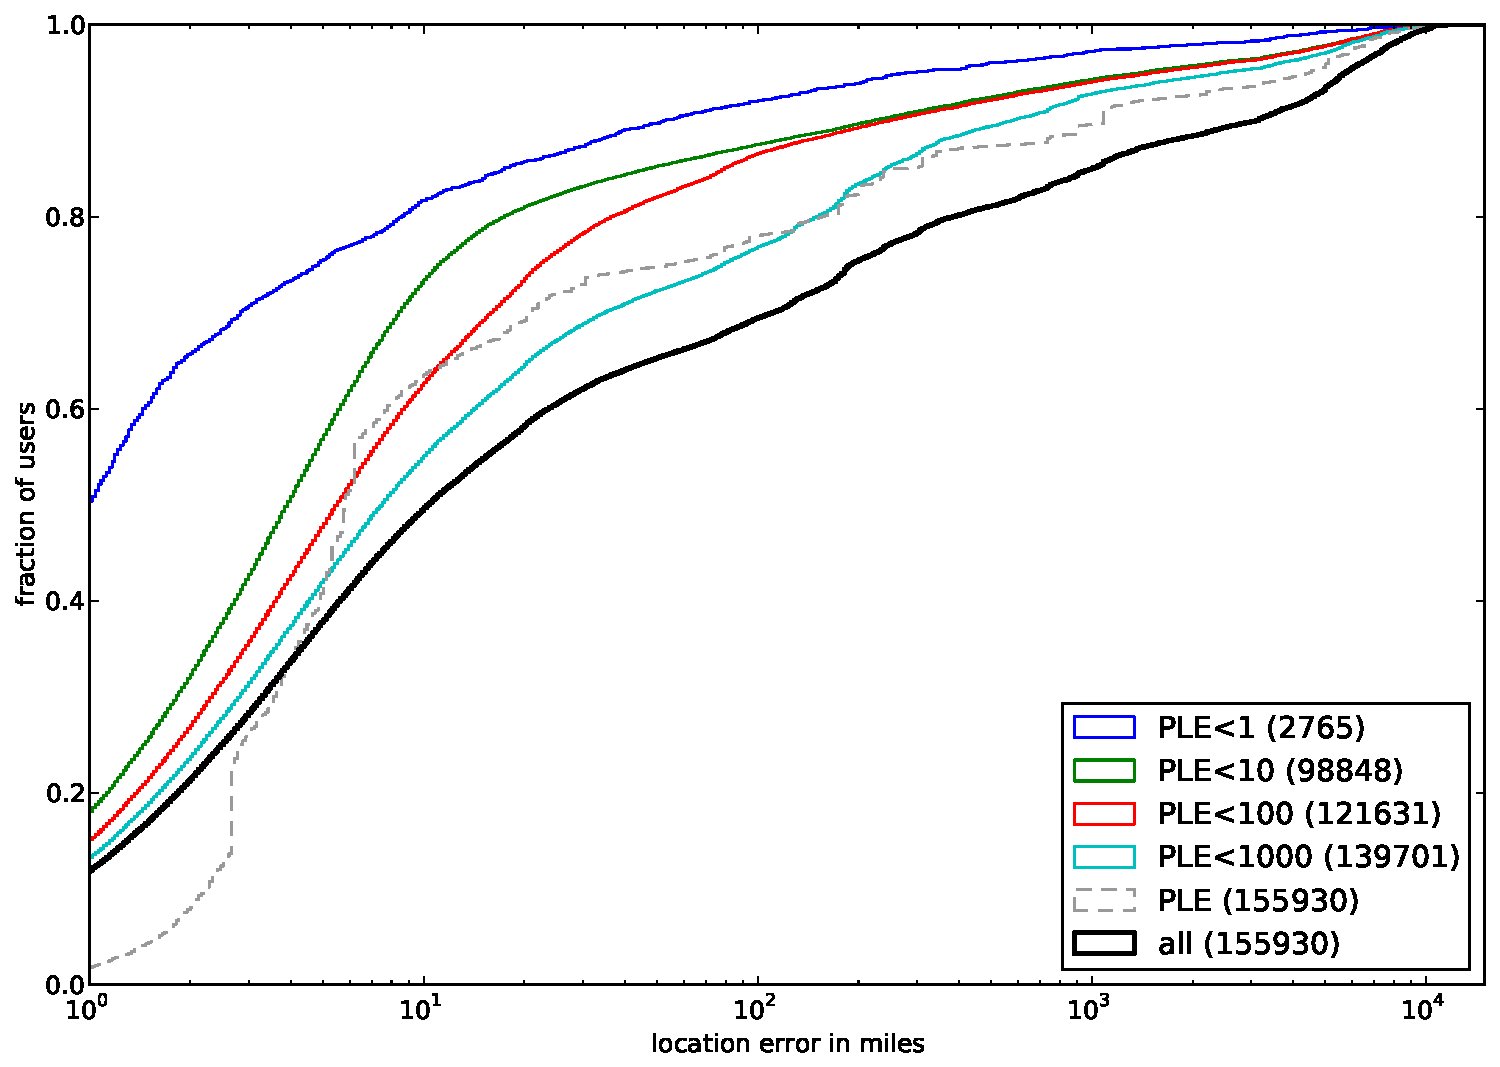
\includegraphics[width=\linewidth]{figures/mloc_mdist.pdf}
\caption{
Cumulative distribution function(CDF) of the distance between geo-located
users' tweets and their geocoded self-reported location.
%
The distances are split into bins based on the median location error(MLE).
%
The blue lines show that locations with a low MLE tend to be accurate, and
locations with a high MLE are rarely accurate.
%
The dotted line shows the values of the MLE for all the
users in this graph.
%
63\% of these users have a MLE less than 10 miles, and 90\% have a MLE
less than 1000.
}
\label{fig:DiffMlocMdist}
\end{figure}

The blue curves in Figure~\ref{fig:DiffMlocMdist} show a comparison of the MLE
and the actual location error for 155,930 of the target users (these are the
target users who also filled out the location field of their profile).
%
90\% of these users have a MLE that is less than 1000 miles.
%
85\% of the target users live within 1000 miles of the location returned by
the geocoder, but after removing only the 10\% of them who have a MLE greater
than 1000 miles, 93\% of the remaining users live within 1000 miles of the
location the geocoder returns.
%
In all of the future experiments, we treat locations with a MLE that is greater
than 1000 as if no location had been supplied.
%
This filters out worthless locations such as ``Pluto'', while keeping somewhat
vague, but still potentially useful locations such as ``California''.
